\documentclass{beamer}[10]
\usepackage{pgf}
\usepackage[english]{babel}
\usepackage[utf8]{inputenc}
\usepackage{beamerthemesplit}
\usepackage{graphics,epsfig, subfigure}
\usepackage{url}
\usepackage{srcltx}
\usepackage{hyperref}
\usepackage{enumitem}

\definecolor{kugreen}{RGB}{50,93,61}
\definecolor{kugreenlys}{RGB}{132,158,139}
\definecolor{kugreenlyslys}{RGB}{173,190,177}
\definecolor{kugreenlyslyslys}{RGB}{214,223,216}
\setbeamercovered{transparent}
\mode<presentation>
\usetheme[numbers,totalnumber,compress,sidebarshades]{PaloAlto}
\setbeamertemplate{footline}[frame number]

\usecolortheme[named=kugreen]{structure}
\useinnertheme{circles}
\usefonttheme[onlymath]{serif}
\setbeamercovered{transparent}
\setbeamertemplate{blocks}[rounded][shadow=true]
\logo{
\includegraphics[width=0.8cm]{../thesis/0_frontmatter/figures/umatlogo}}

%\useoutertheme{infolines} 
\title{Development of an Efficient Public Transport Search Portal for Ghana}
\author[]{Enock Seth Nyamador}
%\supervisor{Dr Hamidu Abdel-Fatao}	
\institute{Computer Science and Engineering Department \\ University of Mines and Technology}
\date{\today}



\begin{document}
	\frame{\titlepage \vspace{-0.5cm}
	}
	
	\frame
	{
		\frametitle{Overview}
		\tableofcontents%[pausesection]
	}
	
	\section{Problem Definition}
	
	\frame{
		\frametitle{PROBLEM DEFINITION}
		\begin{block}{}
			\begin{itemize}[label=$ \circ $]
				\item Road transport is the major means of transportation in Ghana %\citep{aidoo_passengers_2013}
				\item Over $ 95\% $ of all passenger and freight traffic and about $ 97\% $ of all passenger miles in Ghana is by road %\citep{unesco_transportation:_????}
				\item Majority of passengers mostly rely on public transport services; privately owned or corporate taxis, \textit{tro tros} (shared minivans), buses commuting between major cities and other places. 
				%	\item Vast majority of passengers commuting between places mostly rely on public transport services in the form of privately owned or corporate taxis, \textit{tro tros} (shared minivans), buses commuting between major cities.
				\item Difficulty in finding detailed information on transport terminals
			\end{itemize}
		\end{block}
	}


	\frame{
		\frametitle{PROBLEM DEFINITION (CONTD)}
		\begin{block}{}
				%	\begin{figure}
				%	\centering
				%	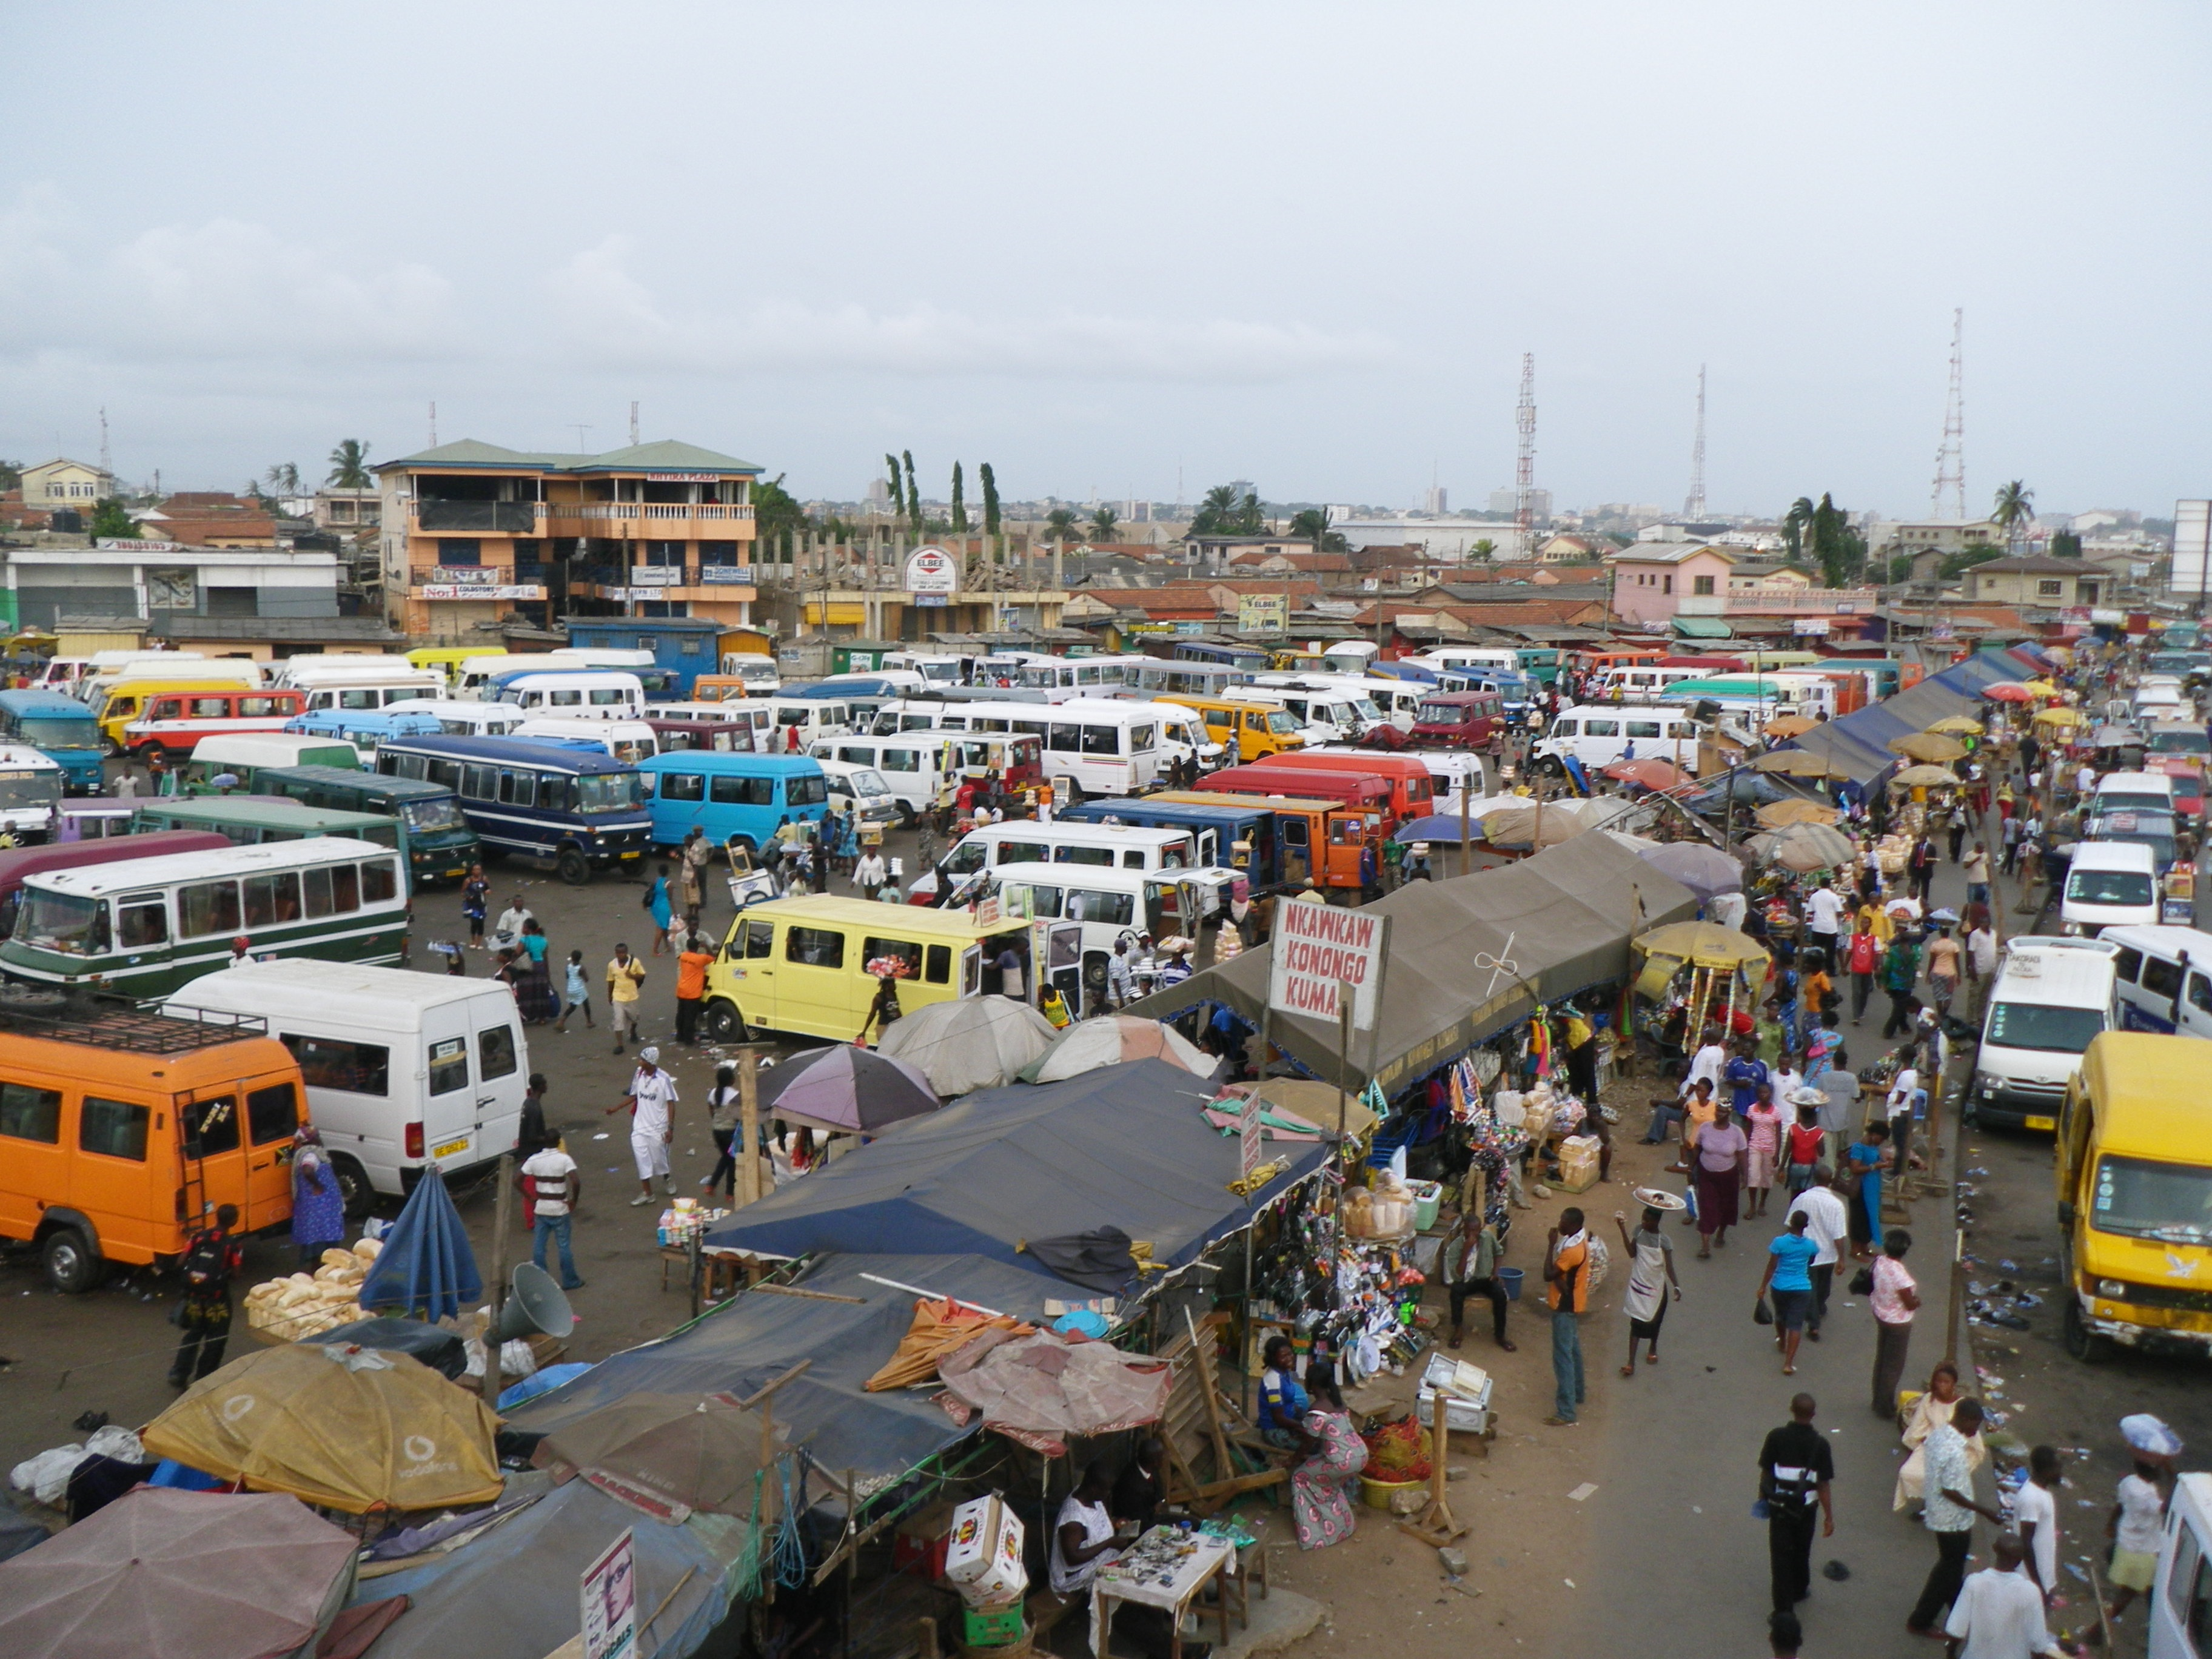
\includegraphics[width=0.7\linewidth]{images/kaneshe}
				%	\caption{Kaneshie Transport Terminal}
				%	\label{fig:kaneshe}
				%	\end{figure}
		\end{block}
	}
		
	
	\frame{
		\frametitle{PROBLEM DEFINITION (CONTD)}
		\begin{block}{}
			%	\begin{figure}
			%	\centering
			%	\includegraphics[width=0.8\linewidth]{images/transport}
			%	\caption{Sample Data Representation}
			%	\label{fig:trasnport}
			%	\end{figure}
	\end{block}
	}

	
	
	\section{Project Objectives}
	\frame{
		\frametitle{PROJECT OBJECTIVES}
		\begin{block}{}
			\begin{itemize}[label=$ \circ $]
				\item To develop a web based public transport terminal search portal that provides detailed information about transport terminals to mitigate the difficulty in finding transport terminals and improve trip planning
			\end{itemize}
		\end{block}
	}
	
	
	\section{Methods used}
	
	\frame{
		\frametitle{METHODS USED}
		\begin{block}{}
			\begin{itemize}[label=$ \circ $]
				\item The system was developed on a local machine %but with scalability and ease of deployment on any kind of infrastructure
				\item The system was developed with Python programming language and Django web framework % If this language proves good enough for deployment purposes it will be used in the final product.	
				\item Survey %to collect information on some transport terminals to facilitate analysis of the existing system
				\item QGIS was used to process and analyze geo-spatial data collected
		\end{itemize}
	\end{block}
	}


	\section{Outcome}

	\frame{
		\frametitle{OUTCOME}
		\begin{block}{}
				\begin{itemize}[label=$ \circ $]
				\item An Internet facing transportation terminal search portal, that provides detailed information about transport terminals available
				%	\item  Possibly generate high definition printer friendly maps that serve nearly same purpose as the web platform
			\end{itemize}	
		\end{block}
	}
		
		
	\section{Facilities used}
		
	\frame{
		\begin{block}{}
			\frametitle{FACILITIES USED}
			\begin{itemize}[label=$ \circ $]
				\item General search engines
				\item Open Data geo-spatial portals with transportation data
				\item Open Source software repositories such as GitHub
				\item PostgresSQL with PostGIS extension
				\item Documentation of any software or libraries used
				\item University of Mines and Technology (UMaT) library
			\end{itemize}
		\end{block}
	}
		
	
\end{document}
